  {\large \fontB Description:}
  
  {\bf solHA} is a 3-dimensional analytical solution to the Cauchy equations with the acceleration term set to zero
  to represent creeping flow. The boundary conditions are free-slip everywhere on a unit domain. 
  The flow is driven by a dense column in the interior. The output from the code is a two-dimensional slice
  at the given height  $z$.
  \\

  {\large \fontB Parameters:}
 
  The variable parameters of this solution are:
  \begin{itemize}
    \item{density parameter: $ \sigma $.}
    \item{viscosity: $\eta$.}
    \item{x width of dense column: $dx$.}
    \item{y width of dense column: $dy$.}
    \item{x centre of dense column: $x0$.}
    \item{y centre of dense column: $y0$.}
    \item{z height of 2D slice: $z$.}
    \end{itemize}

  \begin{SCfigure}[][h]
    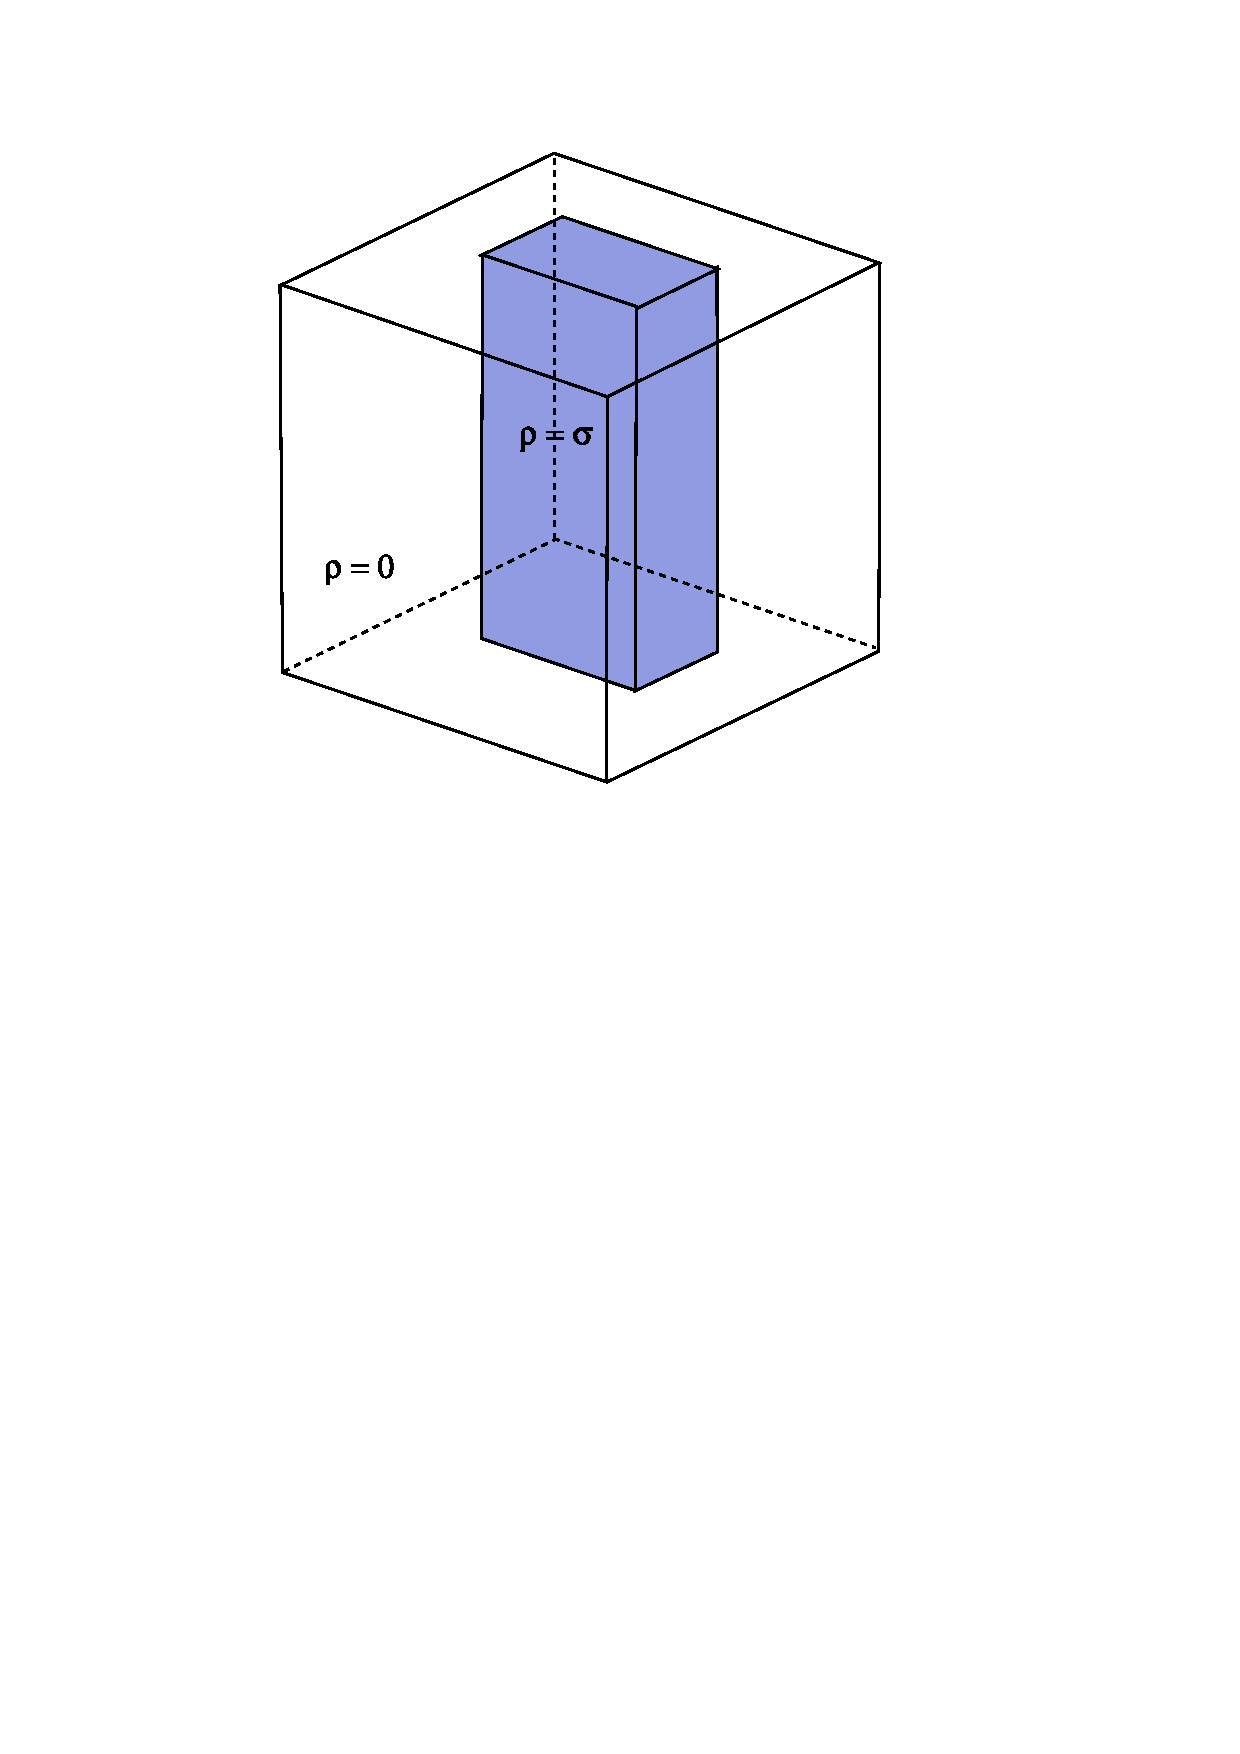
\includegraphics[width=6cm,clip]{../figs/figHA}
    \caption[Short caption]{\label{figHA} 
      Solution ({\bf SolHA}):
      This solution has a block of density $\rho = \sigma$
      of width $dx \times dy$ centred at $x=x0$ and $y=y0$    
       extending in the $z$ direction.
      The boundary conditions are free slip everywhere on the surfaces of the unit box.}
  \end{SCfigure} 
  

